\section{Introduction}
\label{sec:intro}



The age of {\large big data} is upon us as organizations large and small 
are coping with massive volumes of data from sensors, website 
clicks, e-commerce, and more. One such type of big data
problem is in the space of physical simulations (e.g. fluid dynamics,
the $n$-body problem, computer graphics etc.).  This paper investigates 
the specific problem of performing physical simulations
expressed in the language Simit on very large datasets quickly and
deterministically.  Simit generates a static graph, as in \figref{mesh}, 
which is typically
locally connected and embeddable in a $N$D space, where typically
$N=3$.\footnote{We use the notation $N$D to refer to an $N$-dimensional
space.}  Then, a function that operates on each vertex and its neighbors 
is applied to all vertices over many (e.g. at least millions) time steps.
These functions are typically some approximation of physical forces (e.g.
Newton's laws).  Our goal is to develop a software platform that performs these
physical simulations in a fast and scalable manner on a distributed system of 
multi-core nodes.

\begin{wrapfigure}{r}{0.5\textwidth}
\centering
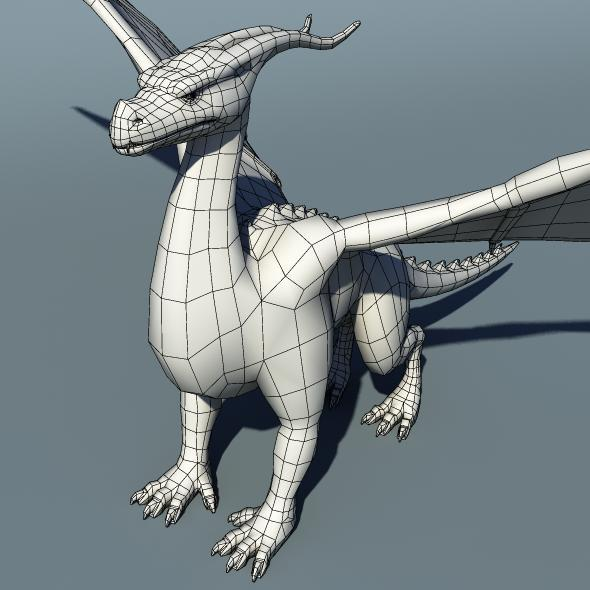
\includegraphics[width=2.5in]{figures/dragon}
\caption{A mesh graph where lines correspond to edges and intersections of lines correspond to vertices.}
\label{fig:mesh}
\end{wrapfigure}



In recent years, there has been 
growing interest in developing frameworks for the storage and 
analysis of this data on large compute clusters, 
Hadoop~\cite{CuttingCa05,DeanGh08} being among among the most 
popular of these. Hadoop breaks up 
large datasets into pieces distributed across many shared-memory
multi-core nodes in a cluster, each of which communicates via
a message-based network protocol. Users supply computations, 
or \defn{map} operators, that are evaluated over each of 
the pieces independently and other computations, or \defn{reduce} 
operators, that combine the results. 
Many problems can be cast into the Hadoop model, but in many 
cases the Hadoop approach is far less effecient than more 
specialized methods, as we will explore throughout this paper.


The idea behind recent big data frameworks, including Hadoop, 
is to decouple scheduling and
data layout from the expression of the computation, enabling high
programmer productivity and portable, best-in-class performance.
However, iterative graph algorithms are one class of problems that
is not well-suited to the Hadoop approach. In particular, each 
Hadoop computation writes its output to disk, so each iteration 
in iterative computations incurs the overhead of a disk write 
and then a subsequent disk read for the next iteration. In 
addition, graphs are difficult to split into completely 
independent sets (with no crossing edges) for the map phase 
of a Hadoop computation, so the maps are often wasteful.
However, the idea of decoupling data and scheduling from the expression of
the algorithm is very useful for designing frameworks
for graph algorithms, even if Hadoop itself is ill-suited to 
the task.  
%Functional programming - more copying
%Fault tolerance - not valued in physical simulation space


%\subheading{Motivation and Problem Definition}




\subsection{Data-graph Computations}

In response to the shortcomings of applying Hadoop and similar systems
to graph problems, 
Guestrin et al developed the GraphLab 
framework~\cite{LowBiGo12} for iterative graph algorithms, 
largely consisting of machine learning algorithms. 
In particular, GraphLab is a framework for implementing a
\defn{data-graph computation}, which consists of a graph $G=(V,E)$,
where each vertex has associated user-specified data and a user-specified 
\defn{update function} which is applied to every vertex, taking
as inputs the data associated with the associated neighbors.  On each
\emph{round} or \emph{time step} the update function is applied to
all vertices.  Many interesting big data algorithms, including Google's 
PageRank, can be easily expressed under this model. GraphLab 
comes in two variants -- a multi-core implementation that 
attains parallelism by updating nodes concurrently on multiple 
processing cores, and a distributed implementation that 
additionally spreads vertices across multi-core nodes.

\subheading{Faster, Determinstic Data-graph Computations}

\begin{figure}[!h]
\centering
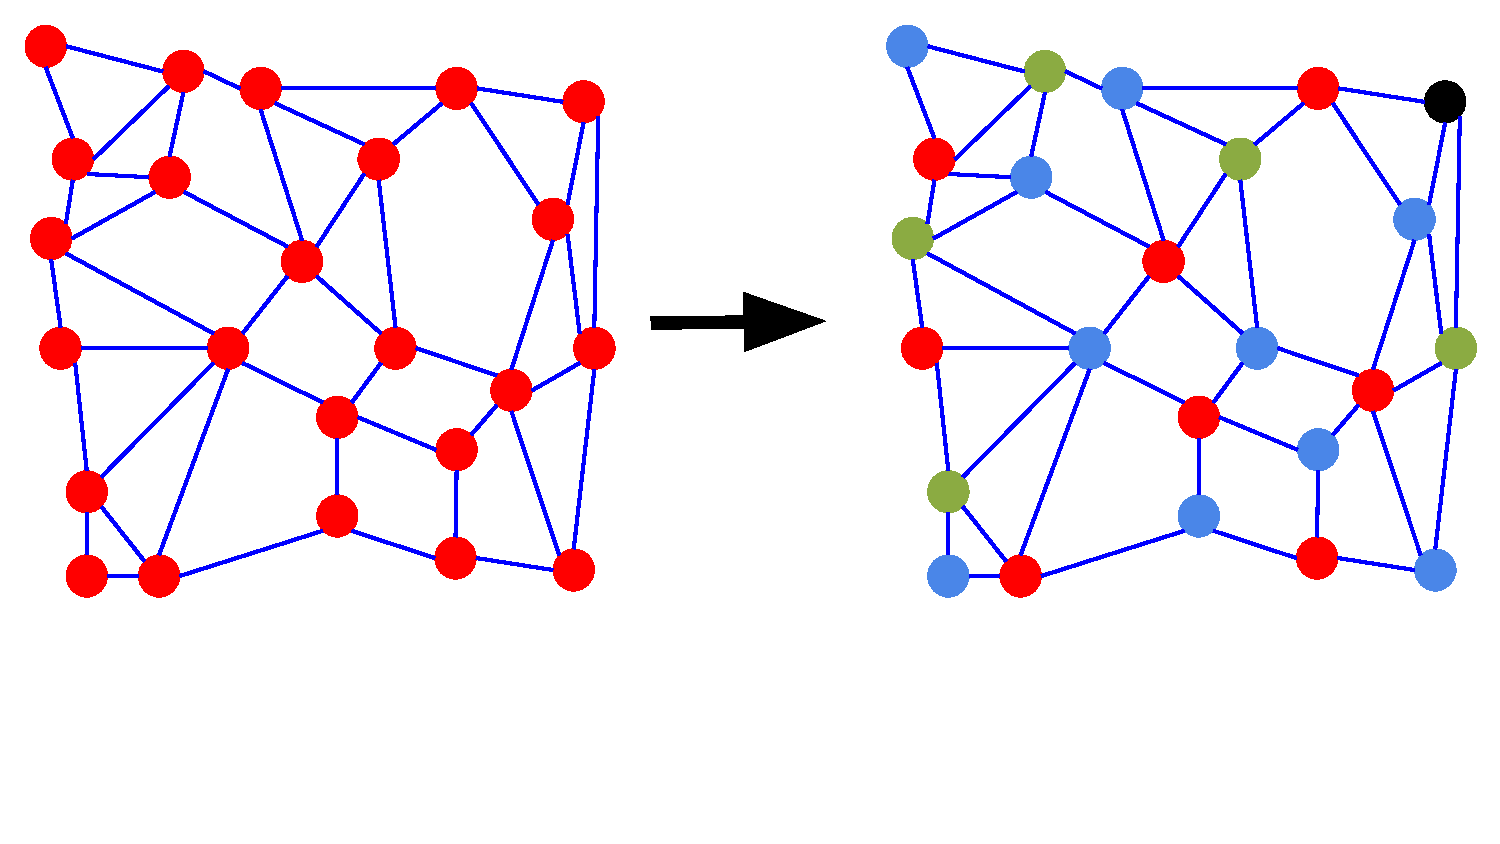
\includegraphics[width=4.5in,clip,trim=0 3cm 0 0]{figures/chromatic_scheduling.pdf}
\caption{Example of how a graph can be partitioned into 
independent sets of vertices denoted by color, each set of which is able to
be executed simultaneously without causing data races.  Iterating
through the colors serially and executing the corresponding
independent sets in parallel is a technique called \emph{chromatic scheduling}.}
\label{fig:chromatic_scheduling}
\end{figure}

Recently, Kaler et al.~\cite{KalerHaSc14} demonstrated that general
data-graph computations could be made to be deterministic without
giving up high-performance, in fact, while increasing performance.
Their system \proc{Prism} is 1.2-2.1 times faster than
the nondeterministic GraphLab framework on a representative suite of data-graph
computations in a multi-core setting.  The technique Kaler et al. proposed
is called \defn{chromatic scheduling}.  In chromatic scheduling one
finds a valid coloring of the graph as depicted in 
\figref{chromatic_scheduling}, an assignment of colors to 
vertices such that no two neighboring vertices share the same color,
and then serializes through the colors.  Since each subset of the graph
of a given color is an independent set (i.e. no two members share an
edge) they may be processed simultaneously without causing a data race.
This assumes that the update function applied to a vertex $v$ reads
the data associated with all of its neighbors 
$\attrib{v}{\id{adj}} = \set{w \in V | \langle v, w \rangle \in E}$ 
and writes only the data
associated with $v$.  Chromatic scheduling is a powerful technique
because it allows the parallel execution of a data-graph computation
without any concurrent operations on data.  This removes the overhead
of mutual-exclusion locks incurred by GraphLab or other atomic operations
that would be required in a design with concurrency.

% As GraphLab and competing frameworks have become more popular, 
% there has been growing interest in optimizing their execution. 
% In the multi-core case, there has been work on reducing 
% costly sychronization steps and more generally on increasing 
% parallelism so that performance can scale up as core counts 
% grow. In the distributed case, the multi-core optimizations 
% have been supplemented by work on more effectively splitting up 
% nodes into sets with few edges between nodes so that expensive 
% inter-node communication can be reduced.
\begin{figure}[!h]
\centering
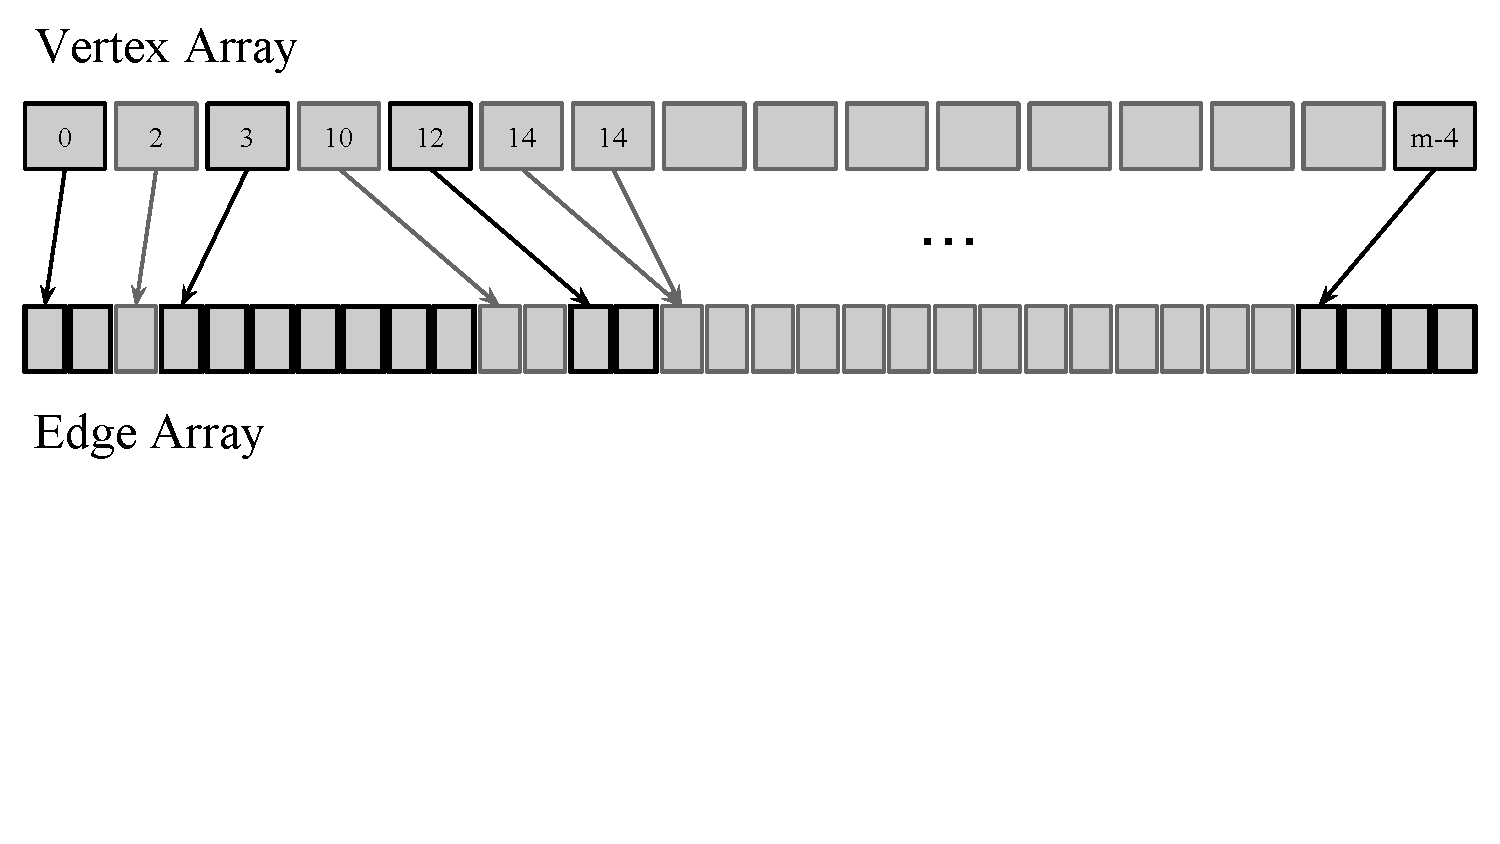
\includegraphics[keepaspectratio,width=4.5in,clip,trim=0 5cm 0 0]{figures/sparse_matrix_representation.pdf}
\caption{Graphs are stored in memory on a single cache-coherent
multi-core in a sparse-matrix format.  The vertex array contains
vertex data and an index into an edge array, which contains vertex
IDs of the associated neighbors.}
\label{fig:layout}
\end{figure}


While chromatic scheduling does a good job of enabling high parallelism
without any concurrency, it can be inefficient for cache usage.  In 
\figref{layout} we see the standard sparse-matrix representation
used in \proc{Prism} and GraphLab.  We can see that to process
the update function of a vertex $v$ of color $c$ the worker needs to read data
associated with all of its neighbors $\attrib{v}{\id{adj}}$, but 
by virtue of being in different color sets by defintion, each
vertex $w \in \attrib{v}{\id{adj}}$ can not be processed until
after all vertices of $c$ have been processed.  This potentially
squanders the potential cache advantage of processing the neighbors
of $v$ soon after $v$ is processed itself, while they are still
in cache.

\begin{figure}[!h]
\centering
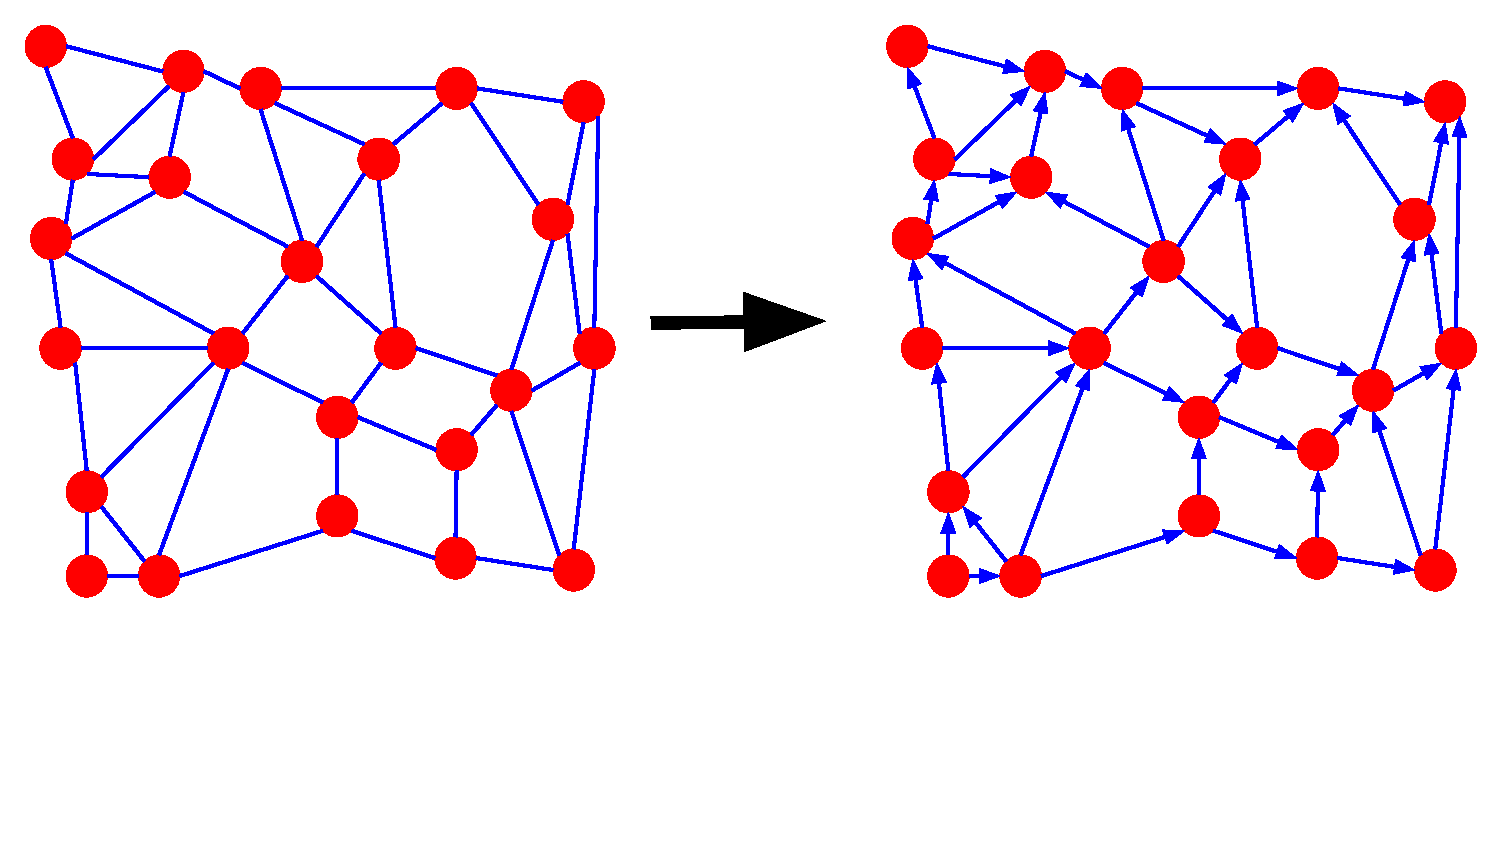
\includegraphics[width=4.5in,clip,trim=0 3cm 0 0]{figures/dag_scheduling.pdf}
\caption{An alternative to chromatic scheduling, which 
yields a deterministic, data race-free output, is dag scheduling.
A priority funcrtion $\rho : V \rightarrow \mathbb{R}$ is used
to create a partial order on the vertices, orienting an edge from
low to high priority results in a 
dag.  The vertices are processed in dag order: a vertex is not
processed until all of its predecessors have been processed.}
\label{fig:dag_scheduling}
\end{figure}

An alternative approach to chromatic scheduling is 
\defn{dag scheduling}~\cite{JonesPl93},
depicted in \figref{dag_scheduling} and used extensively by 
Hasenplaugh et al.~\cite{HasenplaughKaLe14} in the context of graph
coloring.  In dag scheduling, the graph
is turned into a dag through the use of a priority function 
$\rho | V \rightarrow \mathbb{R}$.  In particular, an undirected
edge connecting vertices $v$ and $w$ is oriented as $\langle v, w \rangle$
if $\rho(v) < \rho(w)$ (ties are broken by comparing the vertex numbers).  
The vertices are then processed in dag order, meaning that a vertex
$v$ may be processed only once all of its predecessors 
$\attrib{v}{\id{pred}} = \set{w \in \attrib{v}{\id{adj}} | \rho(w) < \rho(v)}$
have been processed.  A relatively simple implementation of dag
scheduling involves initializing a counter at each vertex with the 
number of predecessors in the dag.  Then, after a vertex $v$ is updated
the worker atomically decrements the counters for all successors 
$\attrib{v}{\id{succ}} = \attrib{v}{\id{adj}} \setminus \attrib{v}{\id{pred}}$,
recursively updating any successors whose counters drop to zero.
This scheduling approach affords us the opportunity
to process vertices shortly after they are read by their neighbors,
a potential caching advantage.  We will explore a technique 
for achieving such cache behavior for a special class of graphs 
corresponding to physical simulations in \secref{hilbert}.



\subsection{Simit}

Simit is a language used to describe physical simulations 
(e.g. fluid dynamics, the $n$-body problem, computer graphics etc.).
Typically, Simit generates a mesh graph (i.e. a wire mesh discretization
of a continuous 3D object) of an object in 
physical 3D space, like the one depicted in \figref{mesh}.  
These meshes contain vertices at intersections of line segments, 
hyperedges (e.g. triangular faces) and tetrahedron volumes, each of which of
these three constructs has associated data.  An immediate hurdle
presents itself when trying to cast operations on such a mesh graph
as a data-graph computation: data-graphs do not natively support
hyperedges or tetrahedra.  However, Simit is a language and thus
the compiler can intervene to represent the mesh graph as a data-graph
where each vertex has a \emph{type}.  We see in \figref{hyperedge}
how a face (or hyperedge) connecting vertices $B$, $D$, and $E$, for example, 
can be represented as a new type of vertex (i.e. the blue squares
in the figure) which is conntected to $B$, $D$, and
$E$ by individual edges.  In addition, a tetrahedron can be 
viewed as a set of four adjacent triangular faces (or hyperedges).  In 
\figref{tetrahedron} we see such an example, where a third type
of vertex (i.e. the purple diamond in the figure) is connected 
to four face type vertices.  Finally, the update function, which
is generated by the Simit compiler can generate an update function
which takes the type of the vertex as a parameter and jumps
to the relevant code as in a case statement.

\begin{figure}[]
\centering
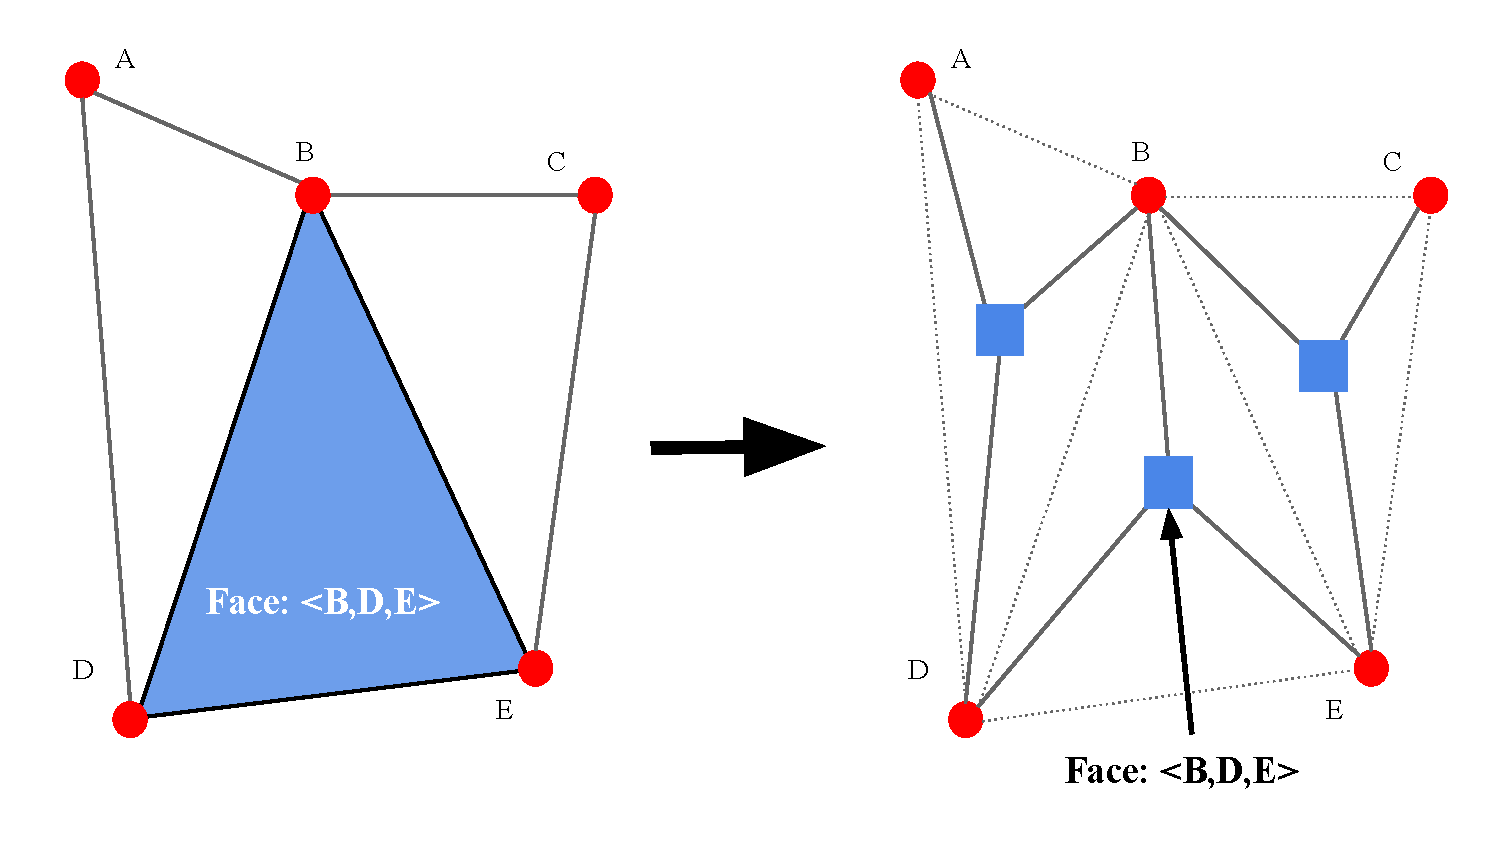
\includegraphics[width=4in]{figures/hyperedge.pdf}
\caption{Graphs generated by the language Simit feature hyperedges, an example
of which is in blue on the left.  Hyperedges are represented by different
\emph{types} of vertices in the resulting data-graph computation.
The square vertices in the figure represent hyperedges and have associated
per-hyperedge data.}
\label{fig:hyperedge}
\end{figure}


\begin{figure}[]
\centering
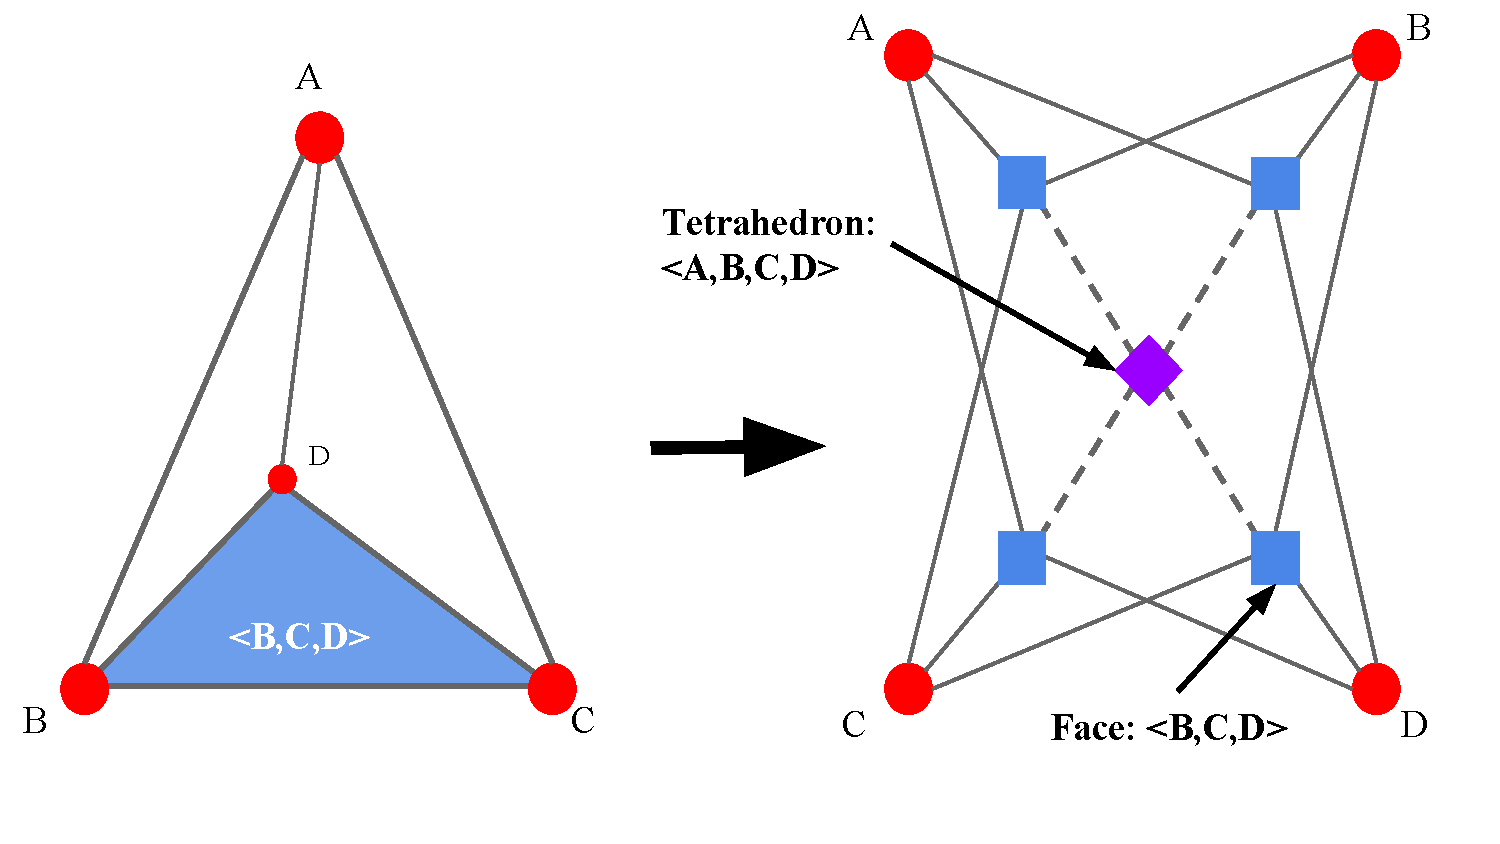
\includegraphics[width=4in]{figures/tetrahedron.pdf}
\caption{Graphs generated by the language Simit have tetrahedrons,
as depicted on the left above.  A tetrahedron is composed of four
hyperedges (or \emph{faces}), an example
of which is in blue on the left.  Tetrahedra are represented by different
\emph{types} of vertices in the resulting data-graph computation.
The diamong vertex on the right represents a tetrahedron and is 
connected to its four constituent hyperedges.}
\label{fig:tetrahedron}
\end{figure}



\subsection{The Hilbert Space-filling Curve}

In this paper we propose a new priority function for 
use with dag scheduling of data-graph computations generated
by Simit.  In particular, we use the bounding box of the
graph in 3D space to normalize the graph to the
unit cube.  Then, we decompose the unit cube into a regular
grid $2^k \times 2^k \times 2^k$ each grid point of which
is assigned a scalar value by the Hilbert space-filling curve~\cite{Hilbert70}.
A 2D example of the Hilbert space-filling
curve is given in \figref{2d_hilbert}.  Then, all vertices
are assigned to the closest grid point and assigned the 
corresponding the scalar value along the Hilbert curve, as
depicted in \figref{hilbert_priority}.  This
scalar value is known as a point's value in \defn{Hilbert space}.  
Since some vertices may be assigned to the same grid point, ties
are broken in the ordering randomly.  Thus, the vertices are 
processed in the order dictated by the Hilbert curve iterating
through the 3D grid.

\begin{SCfigure}
\centering
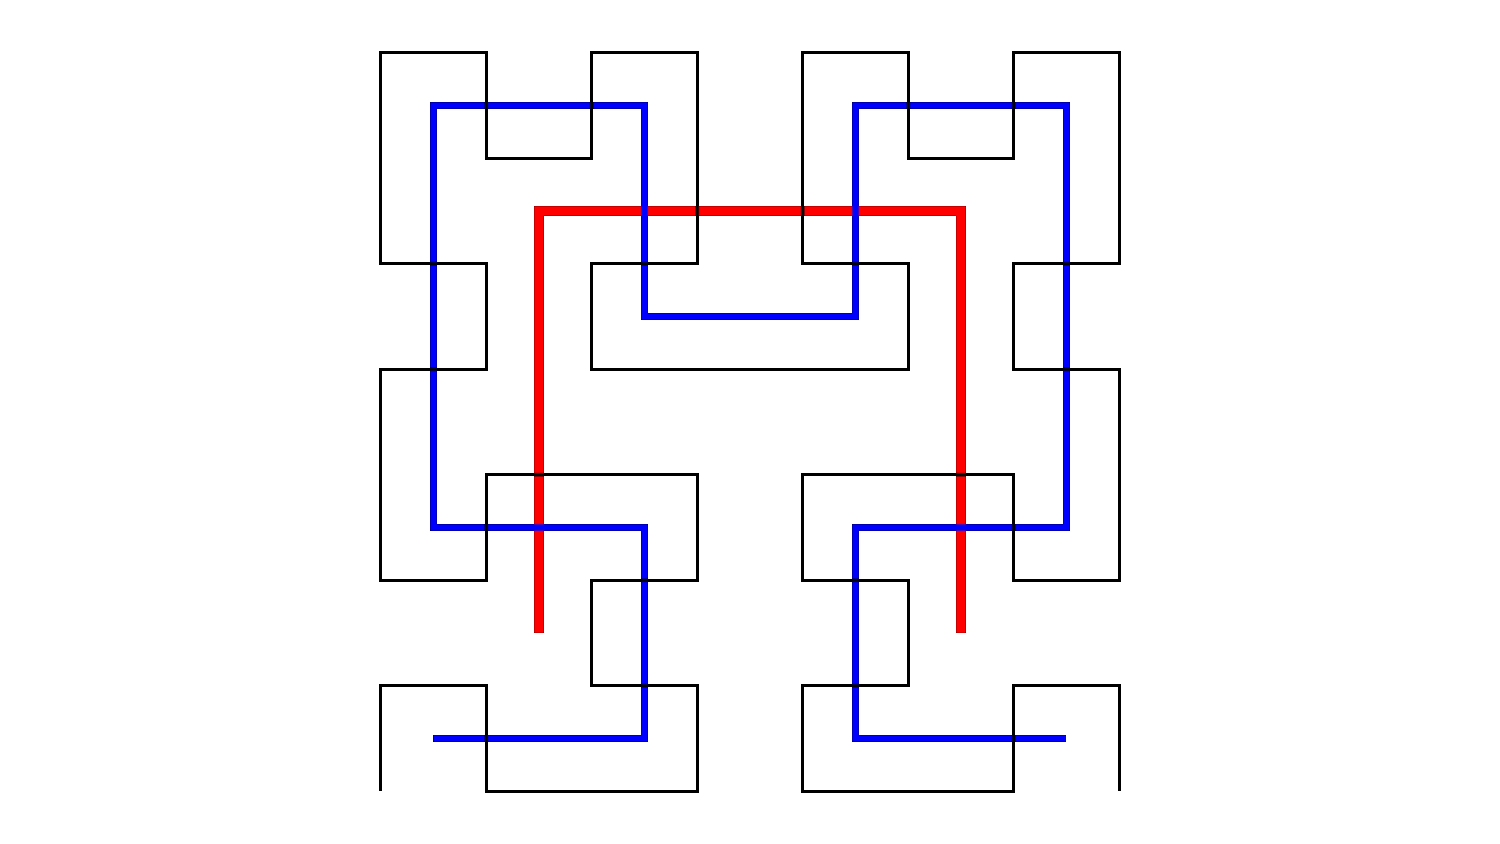
\includegraphics[width=2.5in,clip,trim=4cm 0cm 4cm 0]{figures/2d_hilbert.pdf}
\caption{Three recursion levels of a 2D Hilbert space-filling
curve~\cite{Hilbert70}.  The red curve is the first recursion level and illustrates 
the basic inverted 'U' shape.  The blue curve shows how each quadrant is
partitioned into four independent first-level Hilbert curves (up to 
rotations) of half the size in each dimension.  The black curve
illustrates the third recursion level.}
\label{fig:2d_hilbert}
\end{SCfigure}



Intuitively, one can see why the Hilbert curve might be a good
ordering for the vertices by considering that mesh graphs
are locally connected, meaning that the neighborhood of a vertex
is typically nearby in 3D space.  One well-known property
of the Hilbert curve is that points that are close together
in Hilbert space are also close in 3D space~\cite{GotsmanLi96}.  
However, it is also
true that randomly chosen points that are close together in 
3D space are quite likely to be close in Hilbert space, 
as well~\cite{MoonJaFa96,TirthapuraSeAl06}.
This leads to excellent cache behavior, since the neighbors of
each vertex are close in 3D space for \proc{Simit}-generated mesh graphs,
and will thus tend to also be close in memory.  We call the
priority-dag scheduling algorithm with the Hilbert curve priority
function \proc{Laika}.\footnote{We take naming inspiration from the
graph processing libraries GraphLab~\cite{LowBiGo12},
which is named after a Labrador Retriever, and 
GraphChi~\cite{KyrolaBlGu12}, which
is named after a Chihuahua.  Laika, pictured in \figref{laika}, 
was a Russian street dog that was used in early space 
exploration~\cite{NYT57} and we chose this name
because Laika is a dog who travels through space, much like the Hilbert
curve.}

\begin{wrapfigure}{r}{0.5\textwidth}
\centering
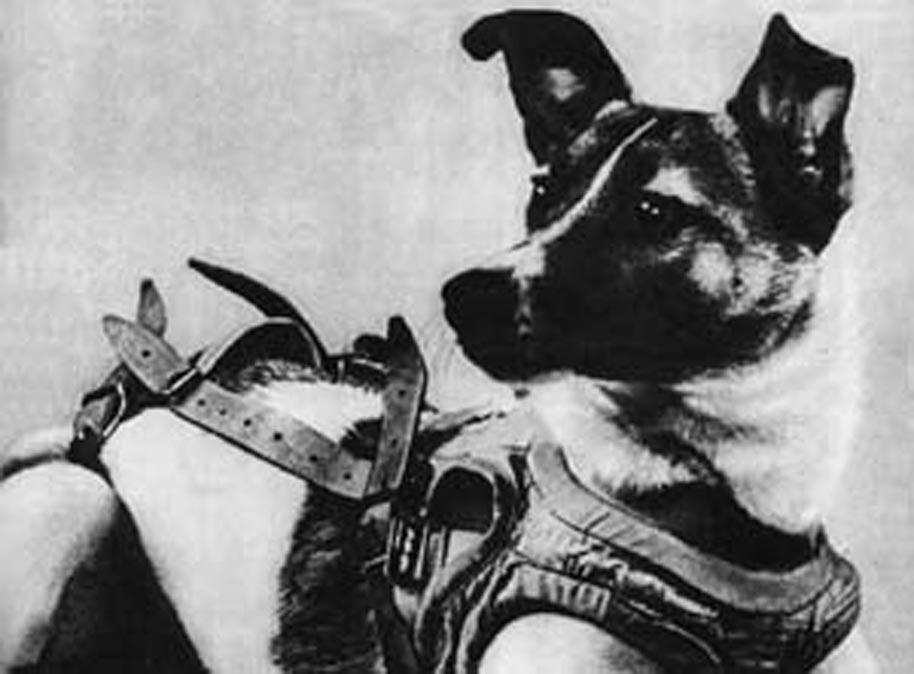
\includegraphics[width=2.5in]{figures/laika.jpg}
\caption{The Russian street dog Laika is one of the first and 
most famous animals to travel through space.}
\label{fig:laika}
\end{wrapfigure}



In addition, the Hilbert curve has another convenient property
that we can exploit toward the goal of partitioning a mesh graph
in distributed memory.  That is, a subinterval in Hilbert space
corresponds to a compact subspace in $N$D space which has a
low surface area to volume ratio~\cite{SinghHoHe93,WarrenSa93,PilkingtonBa96}.  
Since mesh graphs are locally connected, we would then expect 
that the relative number of edges crossing
from one such subspace to another would be low~\cite{MoonJaFa96}.  Thus, to
distributed the computation among $p$ different multi-core
nodes in a distributed system, we merely splic the Hilbert space
evenly in $p$ chunks, while incurring relatively few inter-node
messages.  The use of space-filling curves for locality-preserving 
load-balancing is a well-known technique.  Algorithms 
for the $N$-body problem~\cite{SinghHoHe93,WarrenSa93},
database layout and scheduling~\cite{MoonJaFa96}, 
resource scheduling~\cite{LeungPhJo02}, and dynamic load 
balancing~\cite{HarlacherKlRo12} all use variations on the general
theme of mapping $N$D space onto a 1D curve that is 
subsequently partitioned among $P$ processors.


\subsection{Paper organization}

We will explore the theoretical and experimental 
cache behavior of Hilbert-ordered 
data-graph computations of locally-connected mesh graphs in
\secref{hilbert} and \secref{experimental_results}, respectively.
Then, we will explore the theoretical and experimental
properties of the same class of mesh graphs, albeit much larger,
in \secref{partitions} and \secref{scaling_out}, respectively.
Then, we will offer some concluding remarks in \secref{conclusion}.


\punt{
Citations:
\cite{TirthapuraSeAl06} - analyzes a worst case 3D SFC for probability of 
remote communications for $P = n^\alpha$ for $\alpha \in (0,1)$ for 
communication with neighbors in sphere of constant radius 
$r$: $O(n^{3/4 + \alpha/4})$.  Open question is to analyze 
SFC-specific properties.  Use as main discussion of remote / local.

\cite{HarlacherKlRo12} - uses Z-ordering to adaptively load balance unstructured
meshes where local computations have varying costs - 
this can be referenced as a similar technique for adapting to 
dynamic meshes in future work.

\cite{AluruSe97} - applies the technique of linearizing $N$D space
to 1D space using SFCs, but tackles the problem of data not residing
at discrete locations.  Sorts data using a comparison function that
quickly find the small subspace in SFC that contains both points
thus simplifying the relative comparison in an infinitely recursed SFC
mapping.  Use this to contrast with our technique of merely 'snapping'
each point to its closest point in a fixed grid size.  Note: having a
very fine grid size is not a problem for us and we assume uniform
distribution in space, so tight clustering is not likely.

\cite{GotsmanLi96} - show that if two points are close along the Hilbert
curve they must also be close in Euclidean space.

\cite{LeungPhJo02} - map cores on Computational Plant supercomputer at Sandia
communicating on a 2D toroidal mesh to a 2D Hilbert curve.  
Then, they allocate tasks using a variety of 1D allocation
strategies from the literature.

\cite{WarrenSa93} - introduced a $O(n\lg n)$-time algorithm for calculating
$N$-body forces per time step, given a constant distance cutoff.  
They use a hash table to store particles corresponding to cell in
the oct-tree decomposition of the space, mapped
to 1D via Z-order.  The partition the particles
among the processors by splitting up the SFC-ordered particles
weighted by work.  They state anecdotally that this work allocation
strategy preserves locality.

\cite{SinghHoHe93} - introduced parallel Fast Multipole Method (FMM) 
that decomposes particles using a tree - particles in each of 
a parents children do not interact.  They partition the tree
rather than physical space - dismissing a physical space partitioning
as obviously leading to bad load-balancing.

\cite{PilkingtonBa96} - comparative performance analysis of 
Orthogonal Recursive Bisection (ORB) and Inverse Spacefilling 
Partitioning (ISP) (using Hilbert) load balancing strategies 
for dynamically moving particles.  Empirically observed good
locality.

\cite{MoonJaFa96} - show that the expected number of clusters (subintervals
of a $k$th order $N$-dimensional Hilbert curve) corresponding to a 
random $N$-dimensional polyhedral query $Q$ equals $S/{2N}$ as
$k \rightarrow \infty$, where $S$ is the $N-1$-dimensional 
'surface area' of $Q$.  
}


% -------------------
% Old intro material:

% In this work, we optimize a graph processing framework for a 
% specific workload: physical mesh simulations. A mesh graph 
% is embeddable in 3D space, and an example is shown in Figure 
% 1. Mesh graphs have the nice property that we can partition 
% them into sets corresponding to arbitrary contiguous regions 
% in physical space, and edges cross out of a particular set 
% only from vertices near the boundaries of its physical region. 
% Thus, the number of edges crossing out of a set is proportional 
% to the surface area of its physical region, which is a fairly 
% small quantity relative to the number of vertices, especially 
% when the region has large volume.

% Taking advantage of these properties, we use a novel method 
% based on space-filling curves to split up an input mesh graph 
% across machines to limit inter-machine communication. We then 
% optimize performance on individual machines by evaluating a 
% number of techniques for the scheduling of vertex updates that 
% hit different points in the cache/TLB locality and parallelism 
% design space. Some of our results yield insights for more 
% general classes of graphs.


% Discussion of BSP vs. Gauss-Siedel?







% \subheading{Contributions}

% We anticipate contributing a new technique for and a well-engineered
% implementation of a cache-efficient data-graph computation using
% priority-dag scheduling.  In addition, our implementation will support
% extremely large simulations on distributed-memory clusters.  Both
% of these contributions are high-impact features for the customers
% of Simit, for which \proc{Prism} will be the new backend for multi-cores
% and clusters of multi-cores.  We have some initial exploratory code
% of priority functions (e.g. BFS depth, color).  

% \subheading{Task Breakdown}

% James and Predrag will extend \proc{Prism} to support data reshuffling
% based on a priority per vertex.  Initially, this will be a standalone
% utility that reads a graph file, reorders the vertices and writes out
% the shuffled file.  

% Will and Mohsen will engineer the MPI support for distributed memory,
% including support for distributed data loading.

% \subheading{Issues}

% We descoped our project to focus on being a good back-end for Simit, which
% works on graphs of physical simulations.  This means ditching the investigation
% of software prefetching and static assignment of vertices to processors.
% However, our new focus has allowed us to do something more elegant, essentially
% a cache-oblivious scheduling algorithm for data-graph computations on graphs
% of physical simulations.
